% 
% exemplo genérico de uso da classe iiufrgs.cls
% $Id: iiufrgs.tex,v 1.1.1.1 2005/01/18 23:54:42 avila Exp $
% 
% This is an example file and is hereby explicitly put in the
% public domain.
% 
\documentclass[cic,tc,english]{iiufrgs}
% Para usar o modelo, deve-se informar o programa e o tipo de documento.
% Programas :
% * cic       -- Graduação em Ciência da Computação
% * ecp       -- Graduação em Ciência da Computação
% * ppgc      -- Programa de Pós Graduação em Computação
% * pgmigro   -- Programa de Pós Graduação em Microeletrônica
% 
% Tipos de Documento:
% * tc                -- Trabalhos de Conclusão (apenas cic e ecp)
% * diss ou mestrado  -- Dissertações de Mestrado (ppgc e pgmicro)
% * tese ou doutorado -- Teses de Doutorado (ppgc e pgmicro)
% * ti                -- Trabalho Individual (ppgc e pgmicro)
% 
% Outras Opções:
% * english    -- para textos em inglês
% * openright  -- Força início de capítulos em páginas ímpares (padrão da
% biblioteca)
% * oneside    -- Desliga frente-e-verso
% * nominatalocal -- Lê os dados da nominata do arquivo nominatalocal.def


% Use unicode
\usepackage[utf8]{inputenc}   % pacote para acentuação

% Necessário para incluir figuras
\usepackage{graphicx}         % pacote para importar figuras

\usepackage{listings}

\usepackage{times}            % pacote para usar fonte Adobe Times
% \usepackage{palatino}
% \usepackage{mathptmx}       % p/ usar fonte Adobe Times nas fórmulas

\usepackage[alf,abnt-emphasize=bf]{abntex2cite}	% pacote para usar citações abnt
\newcommand\todo[1]{\textcolor{red}{#1}}

%
% Define o caminho (subpasta) onde você colocará os arquivos de imagem a serem incluídos no texto final
%
\graphicspath{{figures/}} % se tirar fora este comando, por padrão usa a pasta atual

% 
% Informações gerais
% 
\title{Development of a Context Broker with High Availability resource}

\author{Foscarini}{Anderson Didoné}
% alguns documentos podem ter varios autores:
% \author{Flaumann}{Frida Gutenberg}
% \author{Flaumann}{Klaus Gutenberg}

% orientador e co-orientador são opcionais (não diga isso pra eles :))
\advisor[Prof.~Dr.]{Weber}{Taisy Silva}
\coadvisor[M.Sc.]{Crippa}{Marcos Rates}

% a data deve ser a da defesa; se nao especificada, são gerados
% mes e ano correntes
\date{July}{2015}

% o local de realização do trabalho pode ser especificado (ex. para TCs)
% com o comando \location:
\location{Porto Alegre}{RS}

% itens individuais da nominata podem ser redefinidos com os comandos
% abaixo:
% \renewcommand{\nominataReit}{Prof\textsuperscript{a}.~Wrana Maria Panizzi}
% \renewcommand{\nominataReitname}{Reitora}
% \renewcommand{\nominataPRE}{Prof.~Jos{\'e} Carlos Ferraz Hennemann}
% \renewcommand{\nominataPREname}{Pr{\'o}-Reitor de Ensino}
% \renewcommand{\nominataPRAPG}{Prof\textsuperscript{a}.~Joc{\'e}lia Grazia}
% \renewcommand{\nominataPRAPGname}{Pr{\'o}-Reitora Adjunta de P{\'o}s-Gradua{\c{c}}{\~a}o}
% \renewcommand{\nominataDir}{Prof.~Philippe Olivier Alexandre Navaux}
% \renewcommand{\nominataDirname}{Diretor do Instituto de Inform{\'a}tica}
% \renewcommand{\nominataCoord}{Prof.~Carlos Alberto Heuser}
% \renewcommand{\nominataCoordname}{Coordenador do PPGC}
% \renewcommand{\nominataBibchefe}{Beatriz Regina Bastos Haro}
% \renewcommand{\nominataBibchefename}{Bibliotec{\'a}ria-chefe do Instituto de Inform{\'a}tica}
% \renewcommand{\nominataChefeINA}{Prof.~Jos{\'e} Valdeni de Lima}
% \renewcommand{\nominataChefeINAname}{Chefe do \deptINA}
% \renewcommand{\nominataChefeINT}{Prof.~Leila Ribeiro}
% \renewcommand{\nominataChefeINTname}{Chefe do \deptINT}

% A seguir são apresentados comandos específicos para alguns
% tipos de documentos.

% Relatório de Pesquisa [rp]:
% \rp{123}             % numero do rp
% \financ{CNPq, CAPES} % orgaos financiadores

% Trabalho Individual [ti]:
% \ti{123}     % numero do TI
% \ti[II]{456} % no caso de ser o segundo TI

% Monografias de Especialização [espec]:
% \espec{Redes e Sistemas Distribuídos}      % nome do curso
% \coord[Profa.~Dra.]{Weber}{Taisy da Silva} % coordenador do curso
% \dept{INA}                                 % departamento relacionado

% 
% palavras-chave
% iniciar todas com letras minúsculas, exceto no caso de abreviaturas
% 
\keyword{high availability}
\keyword{context broker}
\keyword{context computing}
\keyword{fault tolerance}

%\settowidth{\seclen}{1.10~}

% 
% inicio do documento
% 
\begin{document}

% folha de rosto
% às vezes é necessário redefinir algum comando logo antes de produzir
% a folha de rosto:
% \renewcommand{\coordname}{Coordenadora do Curso}
\maketitle

% dedicatoria
% \clearpage
% \begin{flushright}
%     \mbox{}\vfill
%     {\sffamily\itshape
%       ``If I have seen farther than others,\\
%       it is because I stood on the shoulders of giants.''\\}
%     --- \textsc{Sir~Isaac Newton}
% \end{flushright}

% agradecimentos
%\chapter*{Agradecimentos}
%Agradeço ao \LaTeX\ por não ter vírus de macro\ldots



% resumo na língua do documento
\begin{abstract}
    Context-aware computing is a new and broad area of research in Computer Science. Not many efforts are made towards specific solutions, including related to dependability and fault tolerance. This work aims at developing a Context Broker and proposing the addition of resources that give it High Availability characteristics, taking a first step towards a Dependable Broker.
\end{abstract}

% resumo na outra língua
% como parametros devem ser passados o titulo e as palavras-chave
% na outra língua, separadas por vírgulas
\begin{englishabstract}{Desenvolvimento de Broker de Contexto com Recurso de Alta Disponibilidade}{Alta disponibilidade. broker de contexto. computação de contexto. tolerância a Falhas}
    Computação sensível a contexto é uma nova e ampla área de pesquisa na Ciência da Computação. Não são muitos os esforços em soluções específicas, inclusive as relacionadas à área de tolerância a falhas e confiabilidade.
    Este trabalho tem como objetivo desenvolver um Broker de Contexto e propor a adição e recursos que o dêem características de alta disponibilidade, dando um primeiro passo em direção a um Broker Confiável(Dependable).
\end{englishabstract}

% lista de figuras
\listoffigures

% lista de tabelas
%\listoftables

% lista de abreviaturas e siglas
% o parametro deve ser a abreviatura mais longa
\begin{listofabbrv}{SPMD}
    \item[CxB] Context Broker
    \item[CxC] Context Consumer
    \item[CxP] Context Provider
    \item[REST] Representational State Transfer
\end{listofabbrv}

% idem para a lista de símbolos
% \begin{listofsymbols}{$\alpha\beta\pi\omega$}
%     \item[$\sum{\frac{a}{b}}$] Somatório do produtório
%     \item[$\alpha\beta\pi\omega$] Fator de inconstância do resultado
% \end{listofsymbols}

% sumario
\tableofcontents

% aqui comeca o texto propriamente dito

% inclusion of the chapters
\chapter{Introduction}
\todo{...fill me...}

\begin{itemize}
\item[Motivation]\todo{...fill me...} 

\end{itemize}




The goals of this work are to create a regular Context Broker following previously defined architecture, and to demonstrate the feasibility of the construction of a highly available Context Broker, aiming at a bigger project of a future Dependable Context Broker.

The text is organized as follows: Chapter \ref{chap:definitions} is divided on definitions of Context and Fault Tolerance terms, with Section \ref{sec:context} focusing on the former and Section \ref{sec:fault_tolerance} on the latter. Chapter \ref{chap:implementation} presents the design and implementation of the regular Broker, and the strategies to incorporate High Availability to it. Chapter \ref{chap:tests} shows the tests and comparisons made in this work, and finally Chapter \ref{chap:conclusion} brings the conclusions and future work.
\chapter{Definitions}
This work proposes the application of a high availability technique to a context broker system. For a better understanding of the system and its development, definitions of Context, Context-Aware System, Context Representation, Fault Tolerance and High Availability related terms are presented.

\section{Context}
Context has had many definitions throughout the years. The first time Context was defined regarding the human-computer interaction was by \cite{schilit1994disseminating}, where context is defined related to location, identities of nearby people and objects, and the changes happening to those.  Similarly, \cite{brown1997context} define context as location, people around the user, time of day, season, temperature, etc. Many authors have also defined context using synonyms, as \cite{brown1995stick} had the idea of “environment”, i.e., what the computer knows about the user's environment, or \cite{franklin1998all} that see context as user's situation. Thus, a lot of definitions have existed, but they all end up being too specific. Context is about the whole situation of an application and its users, and we can't really.

\cite{dey2000providing} defined context as follows: ''Context is any information that can be used to characterize the situation of an entity. An entity is a person, place, or object that is considered relevant to the interaction between a user and an application, including the user and application themselves.'' This is the definition this work uses.

\subsection{Context-Aware System}
Like context, context-awareness has had several definitions over the years. The first definition was done by \cite{schilit1994disseminating}, and it restricted to applications informed about context and applications that adapt themselves to context. Later on, synonyms have been used to define a context-aware system: reactive \cite{cooperstock1995evolution}, responsive \cite{elrod1993responsive}, situated \cite{hull1997towards}, context-sensitive  \cite{rekimoto1998augment} and environment-directed \cite{fickas1997software}. All these definitions refer to either using context, adapting to context, or both.

The definition used in this work is provided by \cite{dey2000providing}: ''A system is context-aware if it uses context to provide relevant information and/or services to the user, where relevancy depends on the user's task.''

\subsection{How to represent Context}
According to \cite{dey2000providing}, context-aware applications deal with the who's, where's, when's and what's (the activities that are occurring) of entities, and interpret this information to define why a situation is occurring. The designer of the application must decide what to do with the information. Once we have the information available, either through automated sensors or through user's interference, we need to represent it in a way a machine can process and store it.

\cite{baldauf2007survey} presents and defines the most relevant context modeling options: key-value, markup scheme, graphical, object oriented, logic based and ontology based models. As this work is developed over the same base as \cite{crippa2010}, it uses the same context representation model: a markup scheme variation, ContextML \cite{knappmeyer2010contextml}. It is chosen as it provides **ver artigo do marcos pq escolheu cxml


\subsection{ContextML}

ContextML is an XML-based representation schema for context information, where it is categorized into scopes and related to different types of entities. It is designed to be used with REST-based communication between the framework components \cite{knappmeyer2010contextml}. 

The system consists on three core components: Context Provider, Context Consumer and Context Broker. They are briefly described below, based on definitions made by \cite{knappmeyer2010contextml}. 



\subsubsection{Context Representation}



\subsubsection{Context Provider}
A Context Provider (CxP) provides context information of a certain type, e.g. weather, location, activity, etc. It gathers data from sensors, network, user interactions, or other sources. A CxP is specialized in a specific domain of context information (location, weather etc).


\subsubsection{Context Consumer}
A Context Consumer (CxC) queries for and uses context data, e.g. is a context-aware application. A CxC can retrieve context information asynchronously through a subscription method, or by a synchronous method where it requests the Broker for a specific information or for a particular Provider interface, to query the Provider directly.

\subsubsection{Context Broker}
A Context Broker (CxB) is the central component of the architecture, and is the focus of this work. It handles and aggregates context information, and is an interface between the other architecture components. The CxB allows CxCs to subscribe to context information, and CxPs to provide this information. It also provides a lookup service, where the CxCs can query the CxB for CxPs that have a particular capability, depending on the CxC’s interest.

\subsubsection{Entity and Scope}
An entity is the subject of interest which context data refers to, and it is composed of two parts: a type and an identifier. The type refers to the category of the entity: username for human users, imei for mobile devices, room for a room with sensors, etc. The identifier specifies a particular item within a set of entities of the same type.

A scope is a set of closely related context parameters. Every context parameter has a name and belongs to only one scope. The parameters of a scope can only be requested, updated, provided and store at the same time, making the data always consistent. For example, a scope ‘position’ has latitude, longitude and accuracy attributes; any operation on this scope is performed on all these attributes: if the latitude is updated, so is the longitude and accuracy, what is correct, because otherwise it would not make sense. Entity-scope association is illustrated in Figure \ref{fig:entityscope}. \par

\begin{figure}[H]
	\centering
	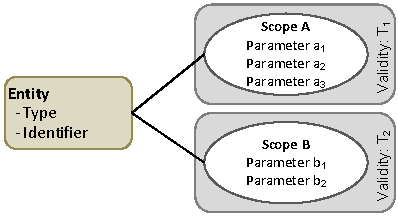
\includegraphics[scale=1]{entityscope.pdf}
	\caption{Entity and Scope relationship. Source: \cite{knappmeyer2010contextml}}
	\label{fig:entityscope}
	
\end{figure}

\subsubsection{Context Messages}


\section{Fault Tolerance}
\subsection{Dependable System}
\subsection{High Availability}
\subsubsection{Uses in real world}
\subsubsection{Problems involving High Availability}


\chapter{Design and Implementation}
\label{chap:implementation}
Bla.

\section{Design and Implementation of the Context Broker}
\label{sec:broker}
This work first implements a regular Context Broker, with no fault tolerance resources. Then, it proposes a strategy to give the Broker High Availability function.
 
\subsection{Platform Choice}
The programming language chosen for the development of this work was Python. Python is a powerful and easy to learn modern programming language \cite{python}. It was chosen because it represents a challenge, and to show that the system is independent of the programmed language, i.e. different applications developed on different programming languages can interact with each other in the architecture, the messages exchanged are what matters. The Python IDE \cite{pycharm} was used, along with GitHub for version control \cite{github}.

The system was implemented over a HTTP REST (Representational State Transfer) Interface. A REST Interface is \cite{fielding2002principled}. For the RESTful implementation, Python Flask framework was used \cite{flask}.

For data persistence, MongoDB was used. MongoDB is a NoSQL 

\subsection{System Architecture}
In Figure \ref{fig:diagram} an overall diagram of the system is illustrated. Each node is a component of the system, and the arrows represent the interaction between them.

\begin{figure}[h]
	\centering
	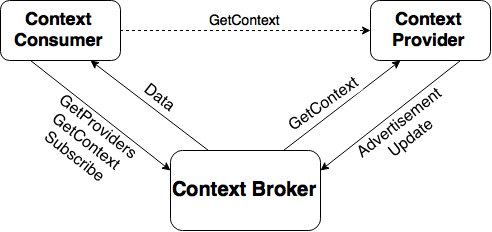
\includegraphics[scale=0.5]{diagram.png}
	\caption{Architecture diagram}
	\label{fig:diagram}
	
\end{figure}


\subsection{Broker Interfaces}
The Context Broker implements several interfaces for communication with the other system components. This section presents each interface and the way they were implemented: what they expect as input (HTTP request from Consumer or Provider), the action they perform, and what they provide as output (response to the Consumer or Provider).


\subsubsection{Advertisement}
\begin{itemize}
	\item[Input:] an Advertisement ContextML message, with Provider information
	
	\item[Action:] registers the Provider within the Broker
	
	\item[Output:] responds the Provider with a ACK or NACK ContextML message, informing success or error, with the corresponding error message.
\end{itemize}

\subsubsection{Update}
\begin{itemize}
	\item[Input:] a ctxEl ContextML Message, with context information to be registered in the Broker
	
	\item[Action:] registers in the Registry Table the context information, with its \textit{contextProvider}, \textit{scope} and \textit{entity} information, \textit{timestamp} and expiration date (\textit{expires}) of the information. It also checks if a \textbf{Subscription} exists for the updated information, sending it to the Consumer \textit{callbackUrl}, when applied.
	
	\item[Output:] responds the Provider with a ACK or NACK ContextML message, informing success or error, with the corresponding error message.
\end{itemize}

\subsubsection{Get Providers}
\begin{itemize}
	\item[Input:] \textit{scope} (mandatory) and \textit{entity type} (optional) arguments in the URL
	
	\item[Action:] looks for registered Providers that provide information matching the arguments given
	
	\item[Output:] responds the Consumer with Providers Lookup ContextML message, containing a list of the providers that match the requested arguments
\end{itemize}

\subsubsection{Get Context}
\begin{itemize}
	\item[Input:] from the Consumer, arguments \textit{scope} and \textit{entity} in the URL
	
	\item[Action:] looks for the latest Context information in the registry that matches the entity and scope received
	
	\item[Output:] responds the Consumer with a ctxEls ContextML message, containing the , or with a NACK ContextML message, informing the error.
	
\end{itemize}
* As seen in Figure \ref{fig:diagram}, there can also exist a direct \textit{GetContext} request from the Consumer to the Provider, thus not involving the Broker. This can be done by the Consumer asking the Broker for a providers list regarding a certain \textit{scope}, and then asking it directly for the desired context information. 

\subsubsection{Subscribe}
\begin{itemize}
	\item[Input:] arguments as follows:  \textit{callbackUrl}, with the URL to where the Broker sends the content it is subscribed to; \textit{scope} and \textit{entity}, with corresponding information the consumer wants to subscribe to; and \textit{minutes}, with the amount of time, in minutes, that the subscription is valid.
	
	\item[Action:] registers the subscription
	
	\item[Output:] responds the Provider with a ACK or NACK ContextML message, informing success or error, with the corresponding error message.
\end{itemize}

\section{Introducing High Availability Technique}
\label{sec:ha_broker}

\subsection{Objective}

\subsection{Design}

\subsection{Protocol created}
Using \cite{protobuf}
\chapter{Tests}
\label{chap:tests}
In this work, the Context Broker was implemented. A Broker management interface was created, it is shown in Figure \ref{fig:broker}. For testing this implementation, both a Provider and a Consumer interfaces were created, respectively illustrated on Figure \ref{fig:provider} and Figure \ref{fig:consumer}.

The Broker management interface allows a system manager to see the Providers registered in the Broker, shown in Figure \ref{fig:providers}, as well as the context information they have updated to it (Figure \ref{fig:registries}). The manager also has access to the Subscriptions made by Consumers and the \textbf{log} of the Broker system, both shown on Figure \ref{fig:subscriptions} and Figure \ref{fig:log}. The figures also illustrate the results of single operations on each interface of the Broker, using the shown Provider and Consumer interfaces. This is for demonstration of the correct functioning of the Broker: a Provider is registered, makes an update and a Consumer makes a subscription and queries the Broker for information the Provider had inserted. These data can be seen on the Providers, Subscriptions and Registry Table web interfaces of the Broker.


The tests performed were simple, regarding only the correct functionality of the Context Broker. The tests should confirm that the Broker operates correctly, without major response delays, and for a considerate amount of time without errors. The correct operation of a Broker consists on it storing and providing Context Data as it is demanded, given well-formed messages from Consumers and Providers.

For the tests, two Context Providers were created, periodically providing location context data, and two Consumers were created, querying the Broker and subscribing for data as well.

The tests results were successful. They were performed on a computer with a Intel(R) Core(TM) i7-3517U CPU @ 1.90GHz processor, 4GB of memory and Fedora release 20 Linux operating system. The Broker was able to manage the requests and the data without major delays, with an average response time of 80ms. 

\begin{figure}[h]
	\centering
	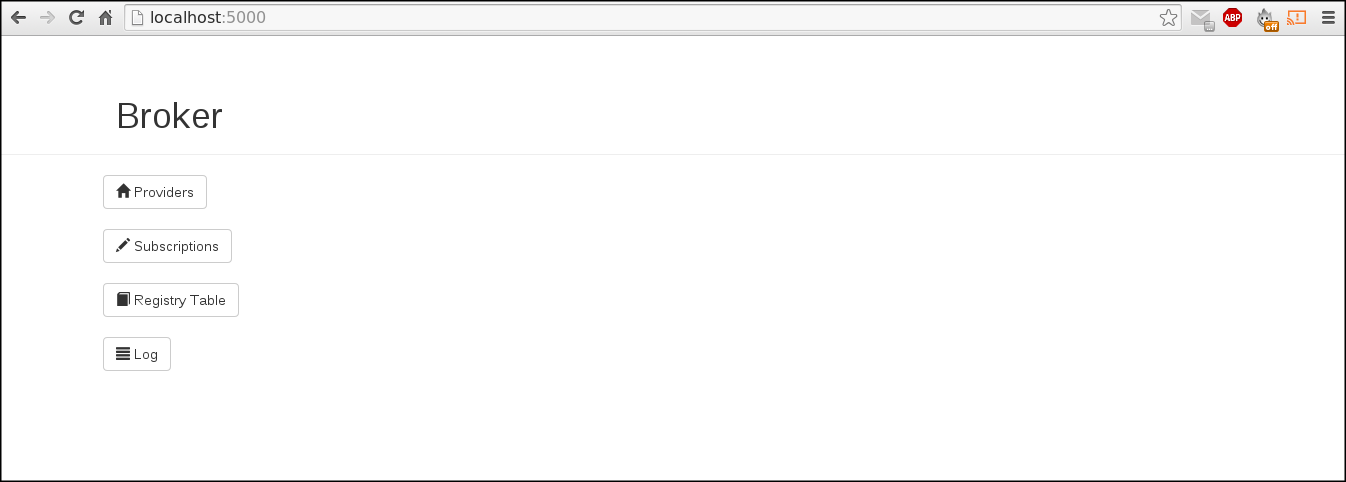
\includegraphics[scale=0.3]{broker.png}
	\caption{Broker Interface}
	\label{fig:broker}
	
\end{figure}

\begin{figure}[h]
	\centering
	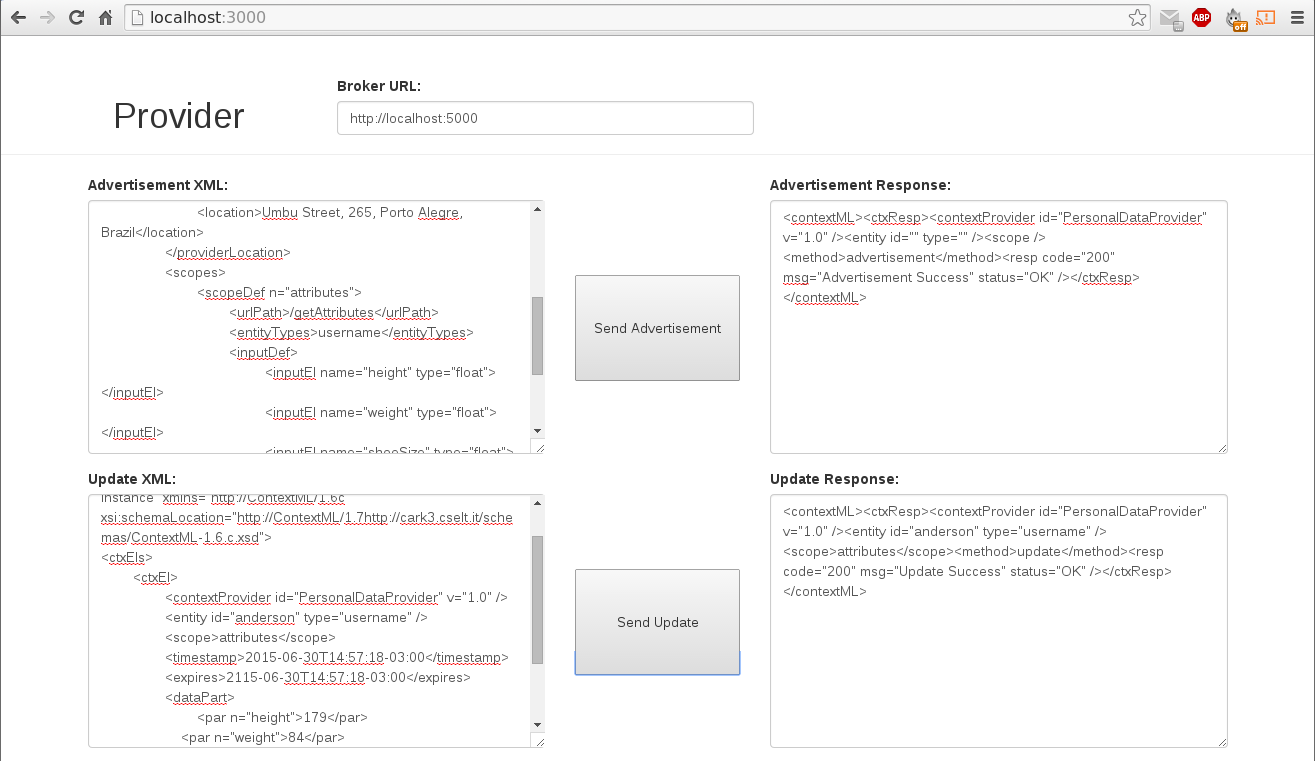
\includegraphics[scale=0.3]{provider.png}
	\caption{Provider Interface}
	\label{fig:provider}
	
\end{figure}

\begin{figure}[h]
	\centering
	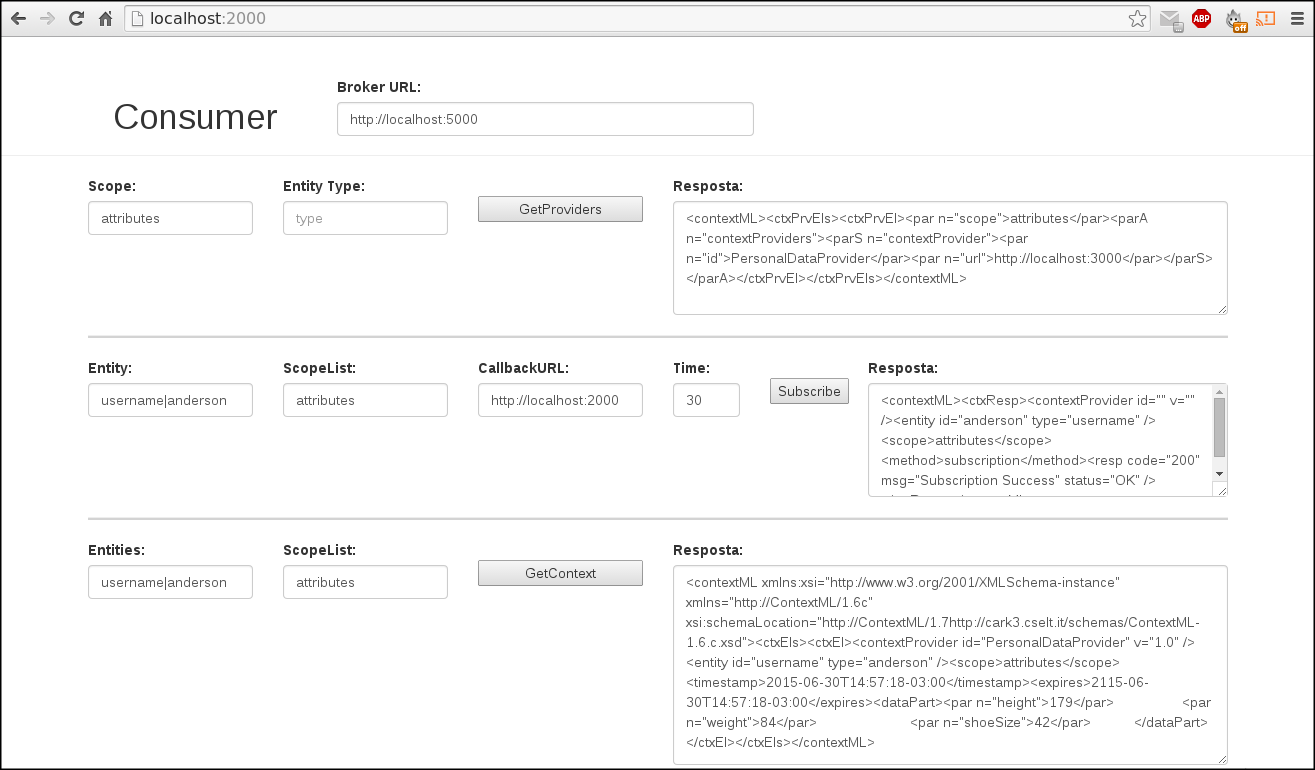
\includegraphics[scale=0.3]{consumer.png}
	\caption{Consumer Interface}
	\label{fig:consumer}
	
\end{figure}

\begin{figure}[h]
	\centering
	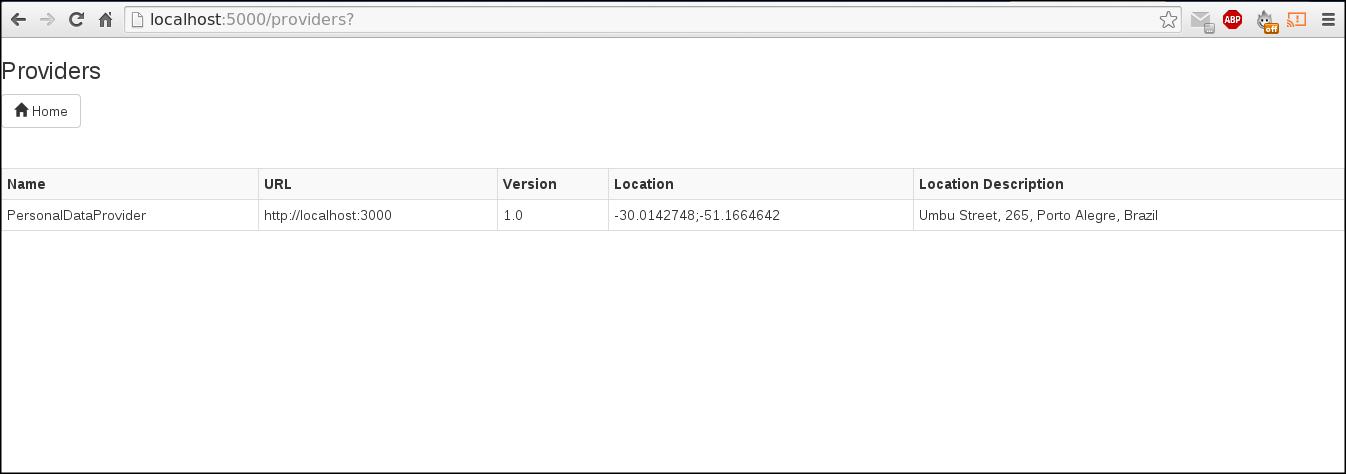
\includegraphics[scale=0.3]{brokerprovs.png}
	\caption{Providers Table}
	\label{fig:brokerprovs}
	
\end{figure}

\begin{figure}[h]
	\centering
	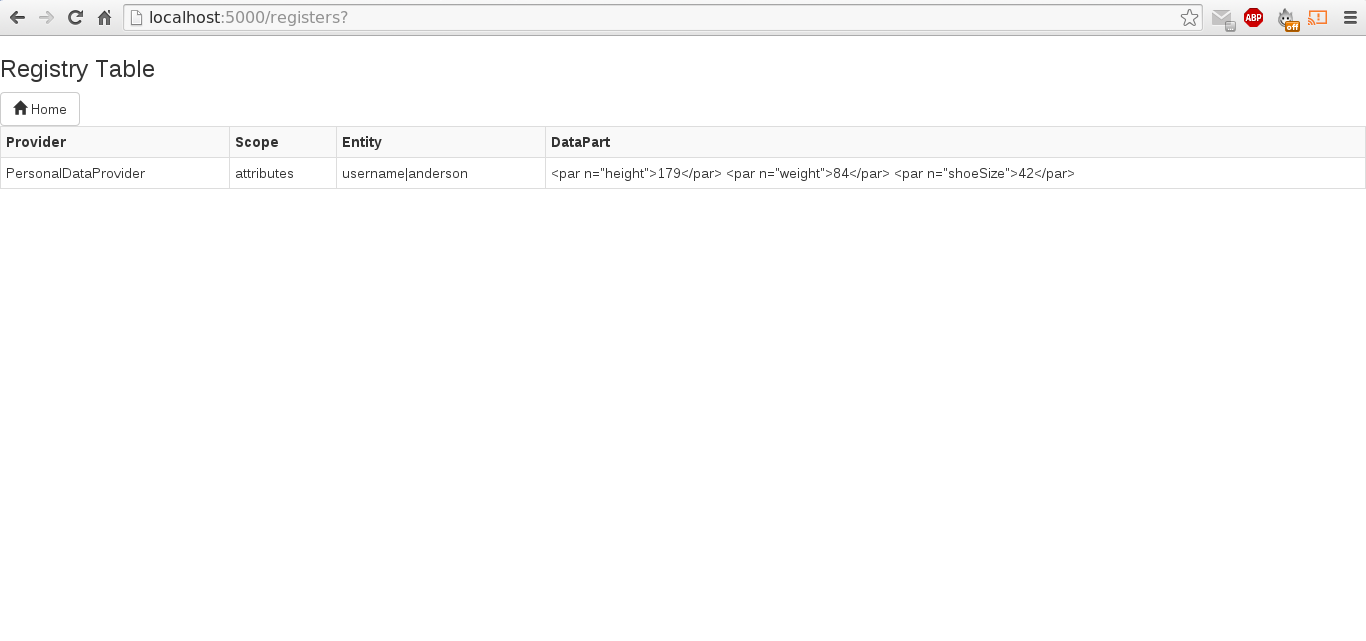
\includegraphics[scale=0.3]{registries.png}
	\caption{Registry Table - Context Information}
	\label{fig:registries}
	
\end{figure}

\begin{figure}[h]
	\centering
	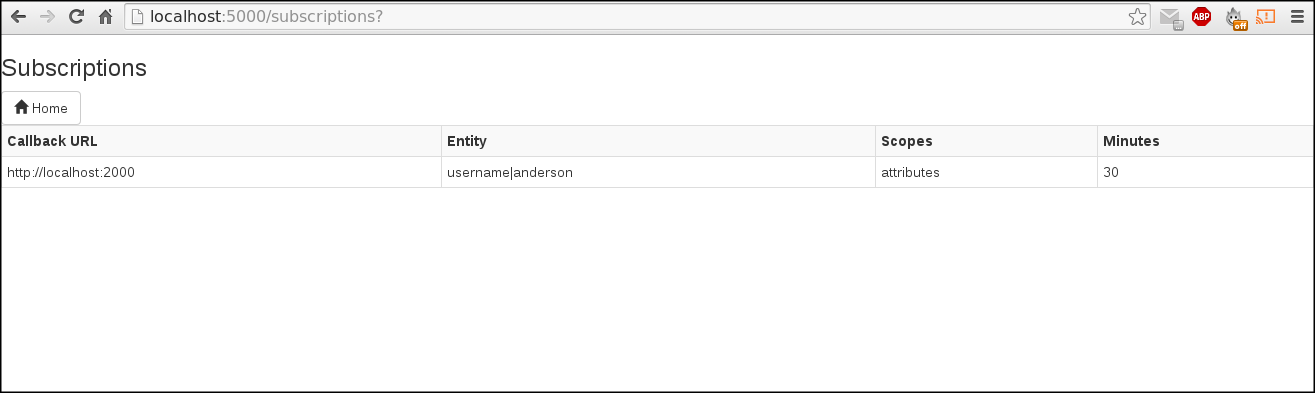
\includegraphics[scale=0.3]{subscriptions.png}
	\caption{Subscriptions Table}
	\label{fig:subscriptions}
	
\end{figure}

\begin{figure}[h]
	\centering
	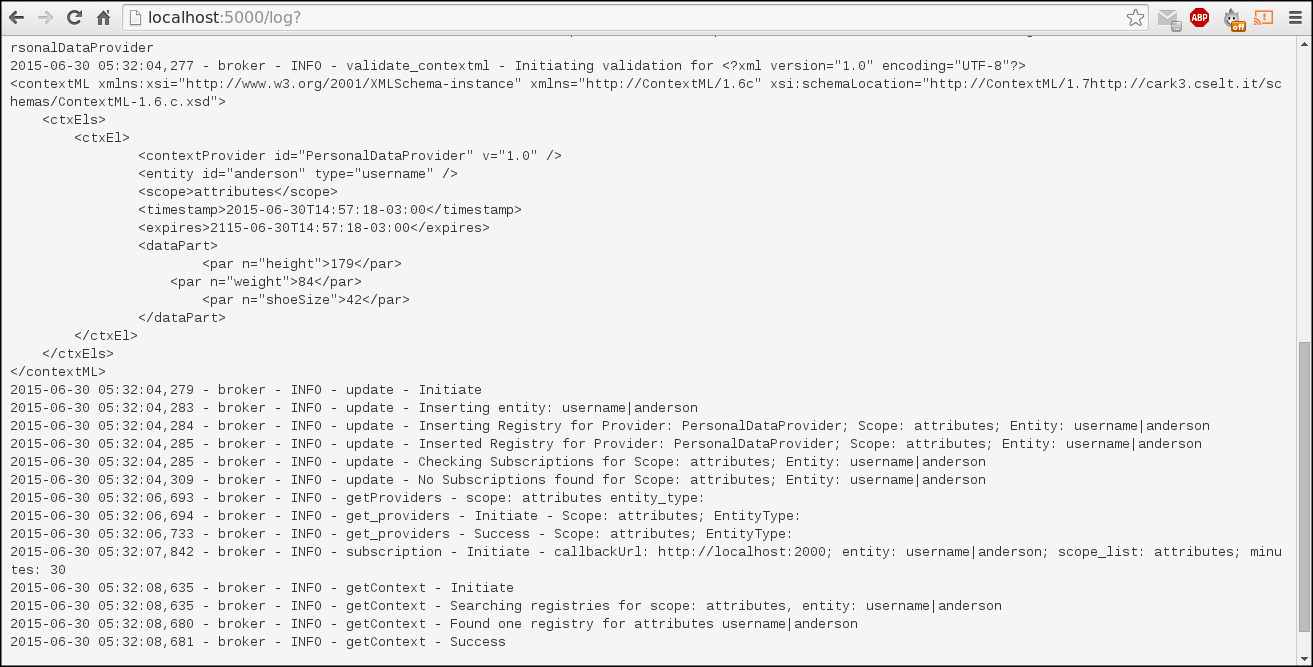
\includegraphics[scale=0.3]{log.png}
	\caption{Broker Log}
	\label{fig:log}
	
\end{figure}

%\todo{perform tests on separate machines, one day execution, create a graph }
\chapter{Conclusion}
Bla.

\section{Future Work}
 


% e aqui vai a parte principal
% 
% \chapter{Estado da arte}
% \chapter{Mais estado da arte}
% \chapter{A minha contribuição}
% \chapter{Prova de que a minha contribuição é válida}
% \chapter{Conclusão}

% referências
% aqui será usado o environment padrao `thebibliography'; porém, sugere-se
% seriamente o uso de BibTeX e do estilo abnt.bst (veja na página do
% UTUG)
% 
% observe também o estilo meio estranho de alguns labels; isso é
% devido ao uso do pacote `natbib', que permite fazer citações de
% autores, ano, e diversas combinações desses

\bibliographystyle{abntex2-alf}
\bibliography{biblio}

\end{document}
